\documentclass[11pt]{article}

\usepackage{minted,xcolor}
\usemintedstyle{monokai}
\definecolor{bg}{HTML}{282828}
\usepackage{xcolor, colortbl}
\usepackage{graphicx}
\usepackage{titlesec}
\usepackage[hmargin=2cm,vmargin=2.5cm]{geometry}
\usepackage{fancyhdr}
\usepackage{hyperref}
\usepackage{caption}
\usepackage{subcaption}

\definecolor{lightblue}{RGB}{174, 199, 232}
\definecolor{lightgrey}{RGB}{232, 232, 232}
\definecolor{tableaublue}{RGB}{78, 121, 167}

\hypersetup{
    colorlinks=true,
    linkcolor=black,
    filecolor=tableaublue,      
    urlcolor=tableaublue,
    pdftitle={Overleaf Example},
    pdfpagemode=FullScreen,
}

\setlength\parindent{0cm}
\setlength\headheight{28pt}

\titleformat{\section}{\normalfont\Large\bfseries}{Part~\thesection:}{6pt}{}[{\titlerule[0.5pt]}]
\titleformat{\subsection}{\normalfont\large\bfseries}{Exercise~\thesubsection:}{6pt}{}

\graphicspath{ {./img/} }

% \title{Practical’s instruction – Networks (week 7)}
% \author{CSC3833 - Data Visualization and Visual Analytic}

\begin{document}

\pagestyle{fancy}
\renewcommand{\headrulewidth}{0pt}
\fancyhead[L]{CSC8626/CSC8642 - Data Visualization}
\fancyhead[R]{2023 / 2024}

\begin{center}
\vspace*{1cm}
{\textbf {\Huge Practical 1}}\\
\vspace*{0.5cm}
{\textbf {\huge Data Encoding}}
\vspace*{1cm}
\end{center}

\section{Physical Visualization}
% ----------------------------------------------------------------------------------------------------------------

This partical focuses on encoding data using is physical objects. You will craft data representations with the use of colour cubes.\\

Form groups of 2 or 3 persons to complete the following assignment.\\

Take time to ask questions and go at your own pace.

\subsection*{Data}

For these exercises you will use the numbers of companies per region (see Figure \ref{fig:map}) and per sector of the North East of England with a focus on the region of Northumberland and Newcaslte (see Table \ref{tab:data}).\\
Source: \href{https://www.ons.gov.uk/businessindustryandtrade/business/activitysizeandlocation/datasets/ukbusinessactivitysizeandlocation}{Office for National Statistics}\\

\begin{figure}[h!]
    \centering
    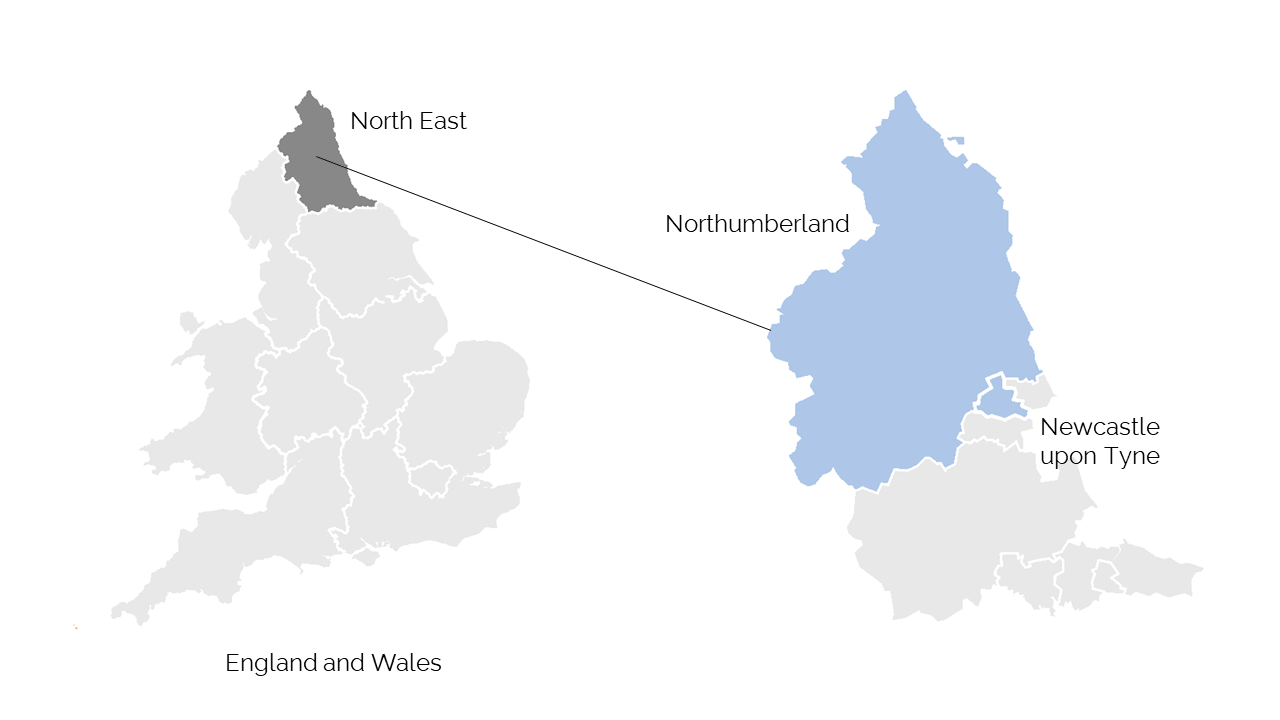
\includegraphics[width=.8\columnwidth]{img/NEmap.png}
    \caption{England and Wales regions, focus on the North East}
    \label{fig:map}
\end{figure}

\begin{table}[h!]
    \centering
{\fontfamily{lmss}\selectfont
\begin{tabular}{|l|l|l|l|l|l|l|l|l|l|}
 \hline
   & \rotatebox[origin=c]{90}{\textbf{Agriculture}} & \rotatebox[origin=c]{90}{\textbf{Information}} \rotatebox[origin=c]{90}{\textbf{\& communication}} & \rotatebox[origin=c]{90}{\textbf{Scientific}} & \rotatebox[origin=c]{90}{\textbf{Health}} & \rotatebox[origin=c]{90}{\textbf{Arts}} \rotatebox[origin=c]{90}{\textbf{\& entertainment}} & \rotatebox[origin=c]{90}{\textbf{Construction}} & \rotatebox[origin=c]{90}{\textbf{Accommodation}} \rotatebox[origin=c]{90}{\textbf{\& food}} & \rotatebox[origin=c]{90}{\textbf{Other}} & \rotatebox[origin=c]{90}{\cellcolor{lightgrey} \textbf{Total}} \\
 \hline
 \textbf{County Durham} & 1,320 & 415 & 1,670 & 515 & 1,015 & 2,255 & 1,345 & 6,190 & \cellcolor{lightgrey}\textbf{14,725} \\
 \hline
 \textbf{Darlington} & 155 & 140 & 495 & 150 & 300 & 455 & 290 & 1,500 & \cellcolor{lightgrey}\textbf{3,485} \\
 \hline
 \textbf{Hartlepool} & 60 & 70 & 390 & 90 & 160 & 355 & 215 & 880 & \cellcolor{lightgrey}\textbf{2,220} \\
 \hline
 \textbf{Middlesbrough} & 20 & 150 & 625 & 175 & 230 & 470 & 325 & 1,465 & \cellcolor{lightgrey}\textbf{3,460} \\
 \hline
 \cellcolor{lightblue}\textbf{Northumberland} & \cellcolor{lightblue}1,845 & \cellcolor{lightblue}380 & \cellcolor{lightblue}1,445 & \cellcolor{lightblue}375 & \cellcolor{lightblue}790 & \cellcolor{lightblue}1,420 & \cellcolor{lightblue}1,060 & \cellcolor{lightblue}4,170 & \cellcolor{lightblue}\textbf{11,485} \\
 \hline
 \textbf{Redcar and Cleveland} & 125 & 80 & 540 & 140 & 240 & 465 & 305 & 1,255 & \cellcolor{lightgrey}\textbf{3,150} \\
 \hline
 \textbf{Stockton-on-Tees} & 90 & 250 & 1,120 & 235 & 400 & 810 & 435 & 2,275 & \cellcolor{lightgrey}\textbf{5,615} \\
 \hline
 \textbf{Tyne and Wear} & 230 & 1,600 & 4,190 & 1,295 & 2,345 & 3,790 & 2,895 & 12,785 & \cellcolor{lightgrey}\textbf{29,130} \\
 \hline
 \textbf{Gateshead} & 60 & 315 & 710 & 250 & 415 & 775 & 445 & 2,640 & \cellcolor{lightgrey}\textbf{5,610} \\
 \hline
 \cellcolor{lightblue}\textbf{Newcastle upon Tyne} & \cellcolor{lightblue}45 & \cellcolor{lightblue}590 & \cellcolor{lightblue}1,480 & \cellcolor{lightblue}450 & \cellcolor{lightblue}775 & \cellcolor{lightblue}890 & \cellcolor{lightblue}930 & \cellcolor{lightblue}3,485 & \cellcolor{lightblue}\textbf{8,645} \\
 \hline
 \textbf{North Tyneside} & 45 & 340 & 860 & 235 & 420 & 730 & 500 & 2,230 & \cellcolor{lightgrey}\textbf{5,360} \\
 \hline
 \textbf{South Tyneside} & 25 & 130 & 490 & 125 & 260 & 510 & 355 & 1,490 & \cellcolor{lightgrey}\textbf{3,385} \\
 \hline
 \textbf{Sunderland} & 55 & 225 & 650 & 235 & 475 & 885 & 665 & 2,940 & \cellcolor{lightgrey}\textbf{6,130} \\
 \hline
 \cellcolor{lightgrey}\textbf{Total}  & \cellcolor{lightgrey}\textbf{4,075} & \cellcolor{lightgrey}\textbf{4,685} & \cellcolor{lightgrey}\textbf{14,665} & \cellcolor{lightgrey}\textbf{4,270} & \cellcolor{lightgrey}\textbf{7,825} & \cellcolor{lightgrey}\textbf{13,810} & \cellcolor{lightgrey}\textbf{9,765} & \cellcolor{lightgrey}\textbf{43,305} & \cellcolor{lightgrey}\textbf{102,400} \\
 \hline
 \cellcolor{lightgrey}\textbf{Total \%} & \cellcolor{lightgrey}\textbf{4\%} & \cellcolor{lightgrey}\textbf{5\%} & \cellcolor{lightgrey}\textbf{14\%} & \cellcolor{lightgrey}\textbf{4\%} & \cellcolor{lightgrey}\textbf{8\%} & \cellcolor{lightgrey}\textbf{13\%} & \cellcolor{lightgrey}\textbf{10\%} & \cellcolor{lightgrey}\textbf{42\%} & \cellcolor{lightgrey}\textbf{100\%} \\
 \hline
\end{tabular}
}
    \caption{2022 number of companies in the North East of England per sector}
    \label{tab:data}
\end{table}

\subsection*{Material}

Utilize the coloured cubes provided in the practical room to construct your visualizations (see Figure \ref{fig:cubes}). There are a total of 10 distinct colors at your disposal: yellow, red, blue, green, orange, pink, purple, black, white, and brown.\\

For legends, use transparent sheets, pens, and erasers that are located next to the cubes (see Figure \ref{fig:sheets}).

\begin{figure}[h!]
    \centering
    \begin{minipage}{.5\textwidth}
      \centering
      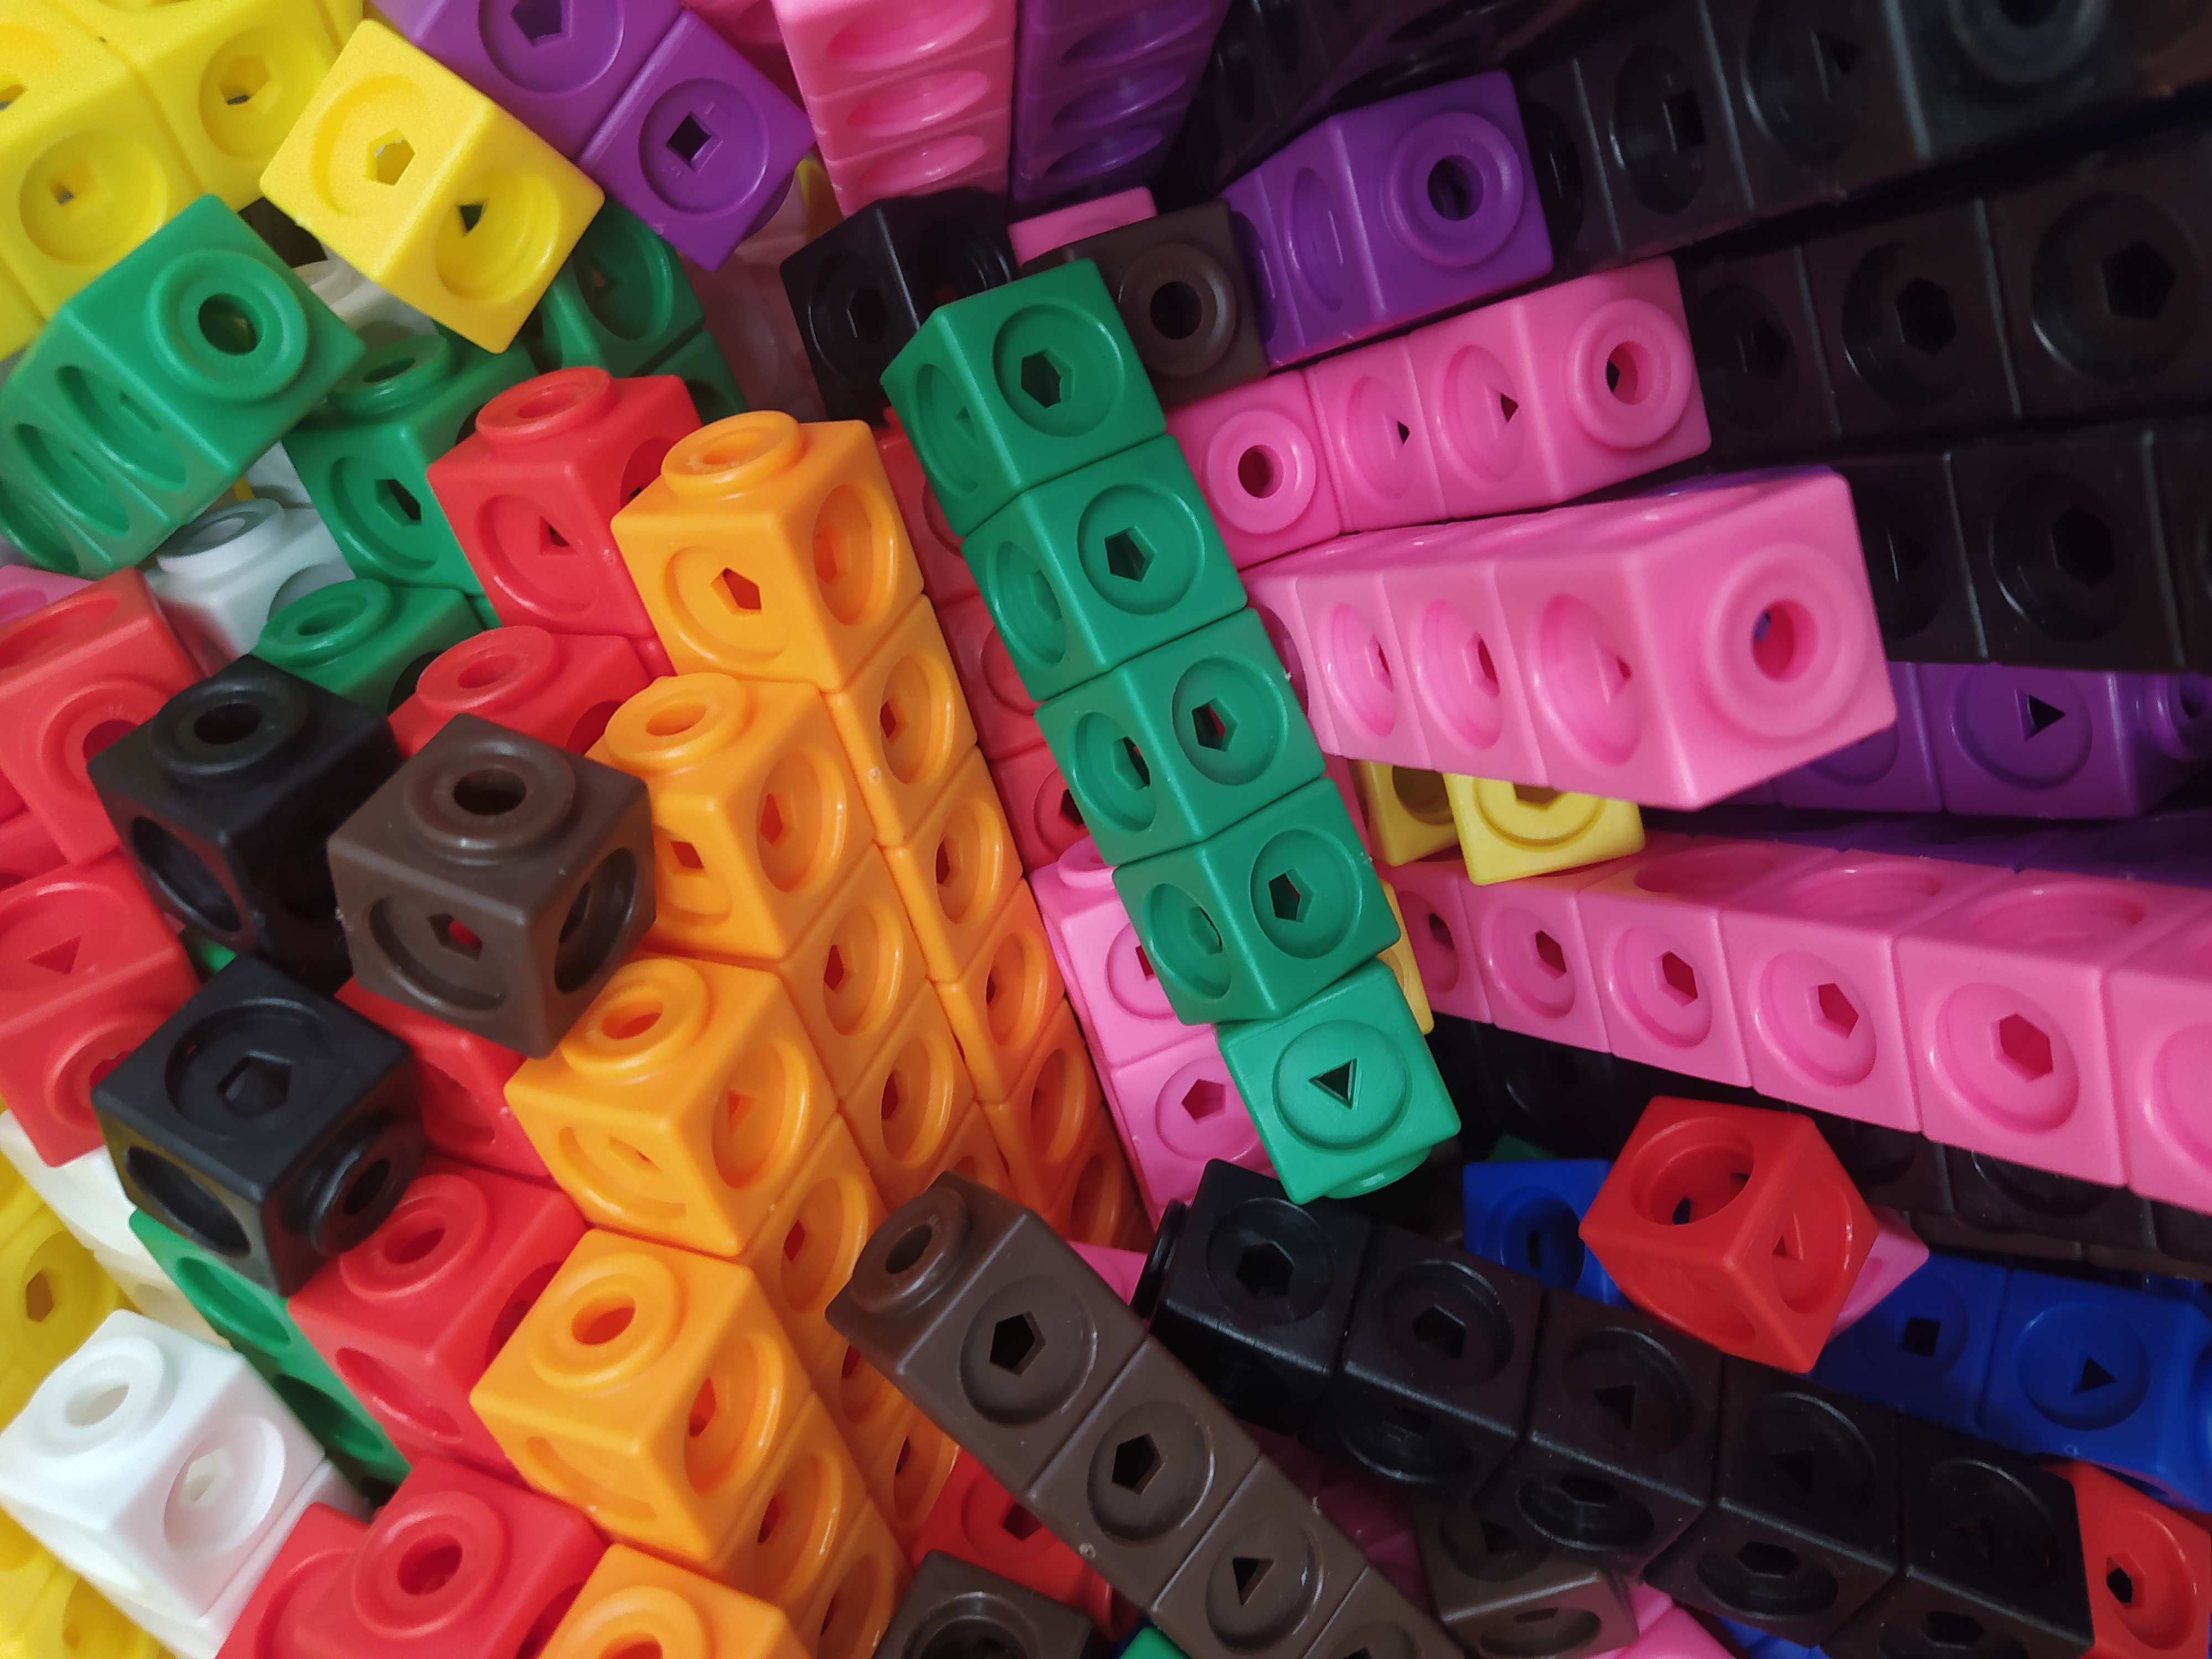
\includegraphics[width=.8\linewidth]{img/physicalCubes.jpg}
      \captionof{figure}{Coloured cubes}
      \label{fig:cubes}
    \end{minipage}%
    \begin{minipage}{.5\textwidth}
      \centering
      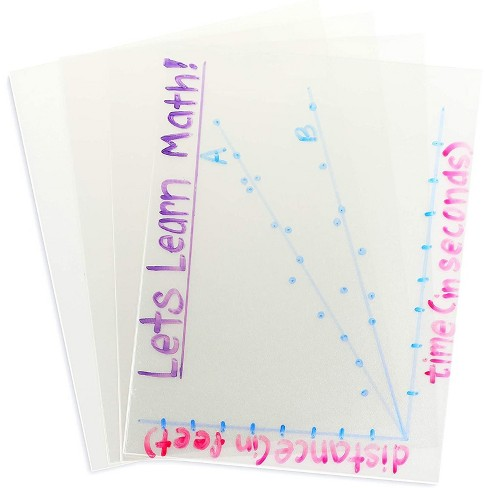
\includegraphics[width=.6\linewidth]{img/transparentSheets.jpg}
      \captionof{figure}{Transparent sheets}
      \label{fig:sheets}
    \end{minipage}
\end{figure}

\subsection{North East companies per sector}

Create a visualization that represents the numbers of companies per sector in the North East.\\

Consider the nature of the data and select which visual variables would be the most suitable for representing them, such as color, size, position, and so on. Think about the scale of your representation. Try to use a maximum of 10 cubes per colour. Finally, think about incorporating a legend. Describe how each visual variable and scale will be utilized, and ensure you include a clear and explicit title for your visualization.\\

Tips:
\begin{itemize}
    \item Use one cube for 4,000 companies
\end{itemize}

Before proceeding to the next exercise, share your work with a demonstrator to receive feedback and guidance.\\

\underline{Expected result}

\begin{figure}[h!]
    \centering
    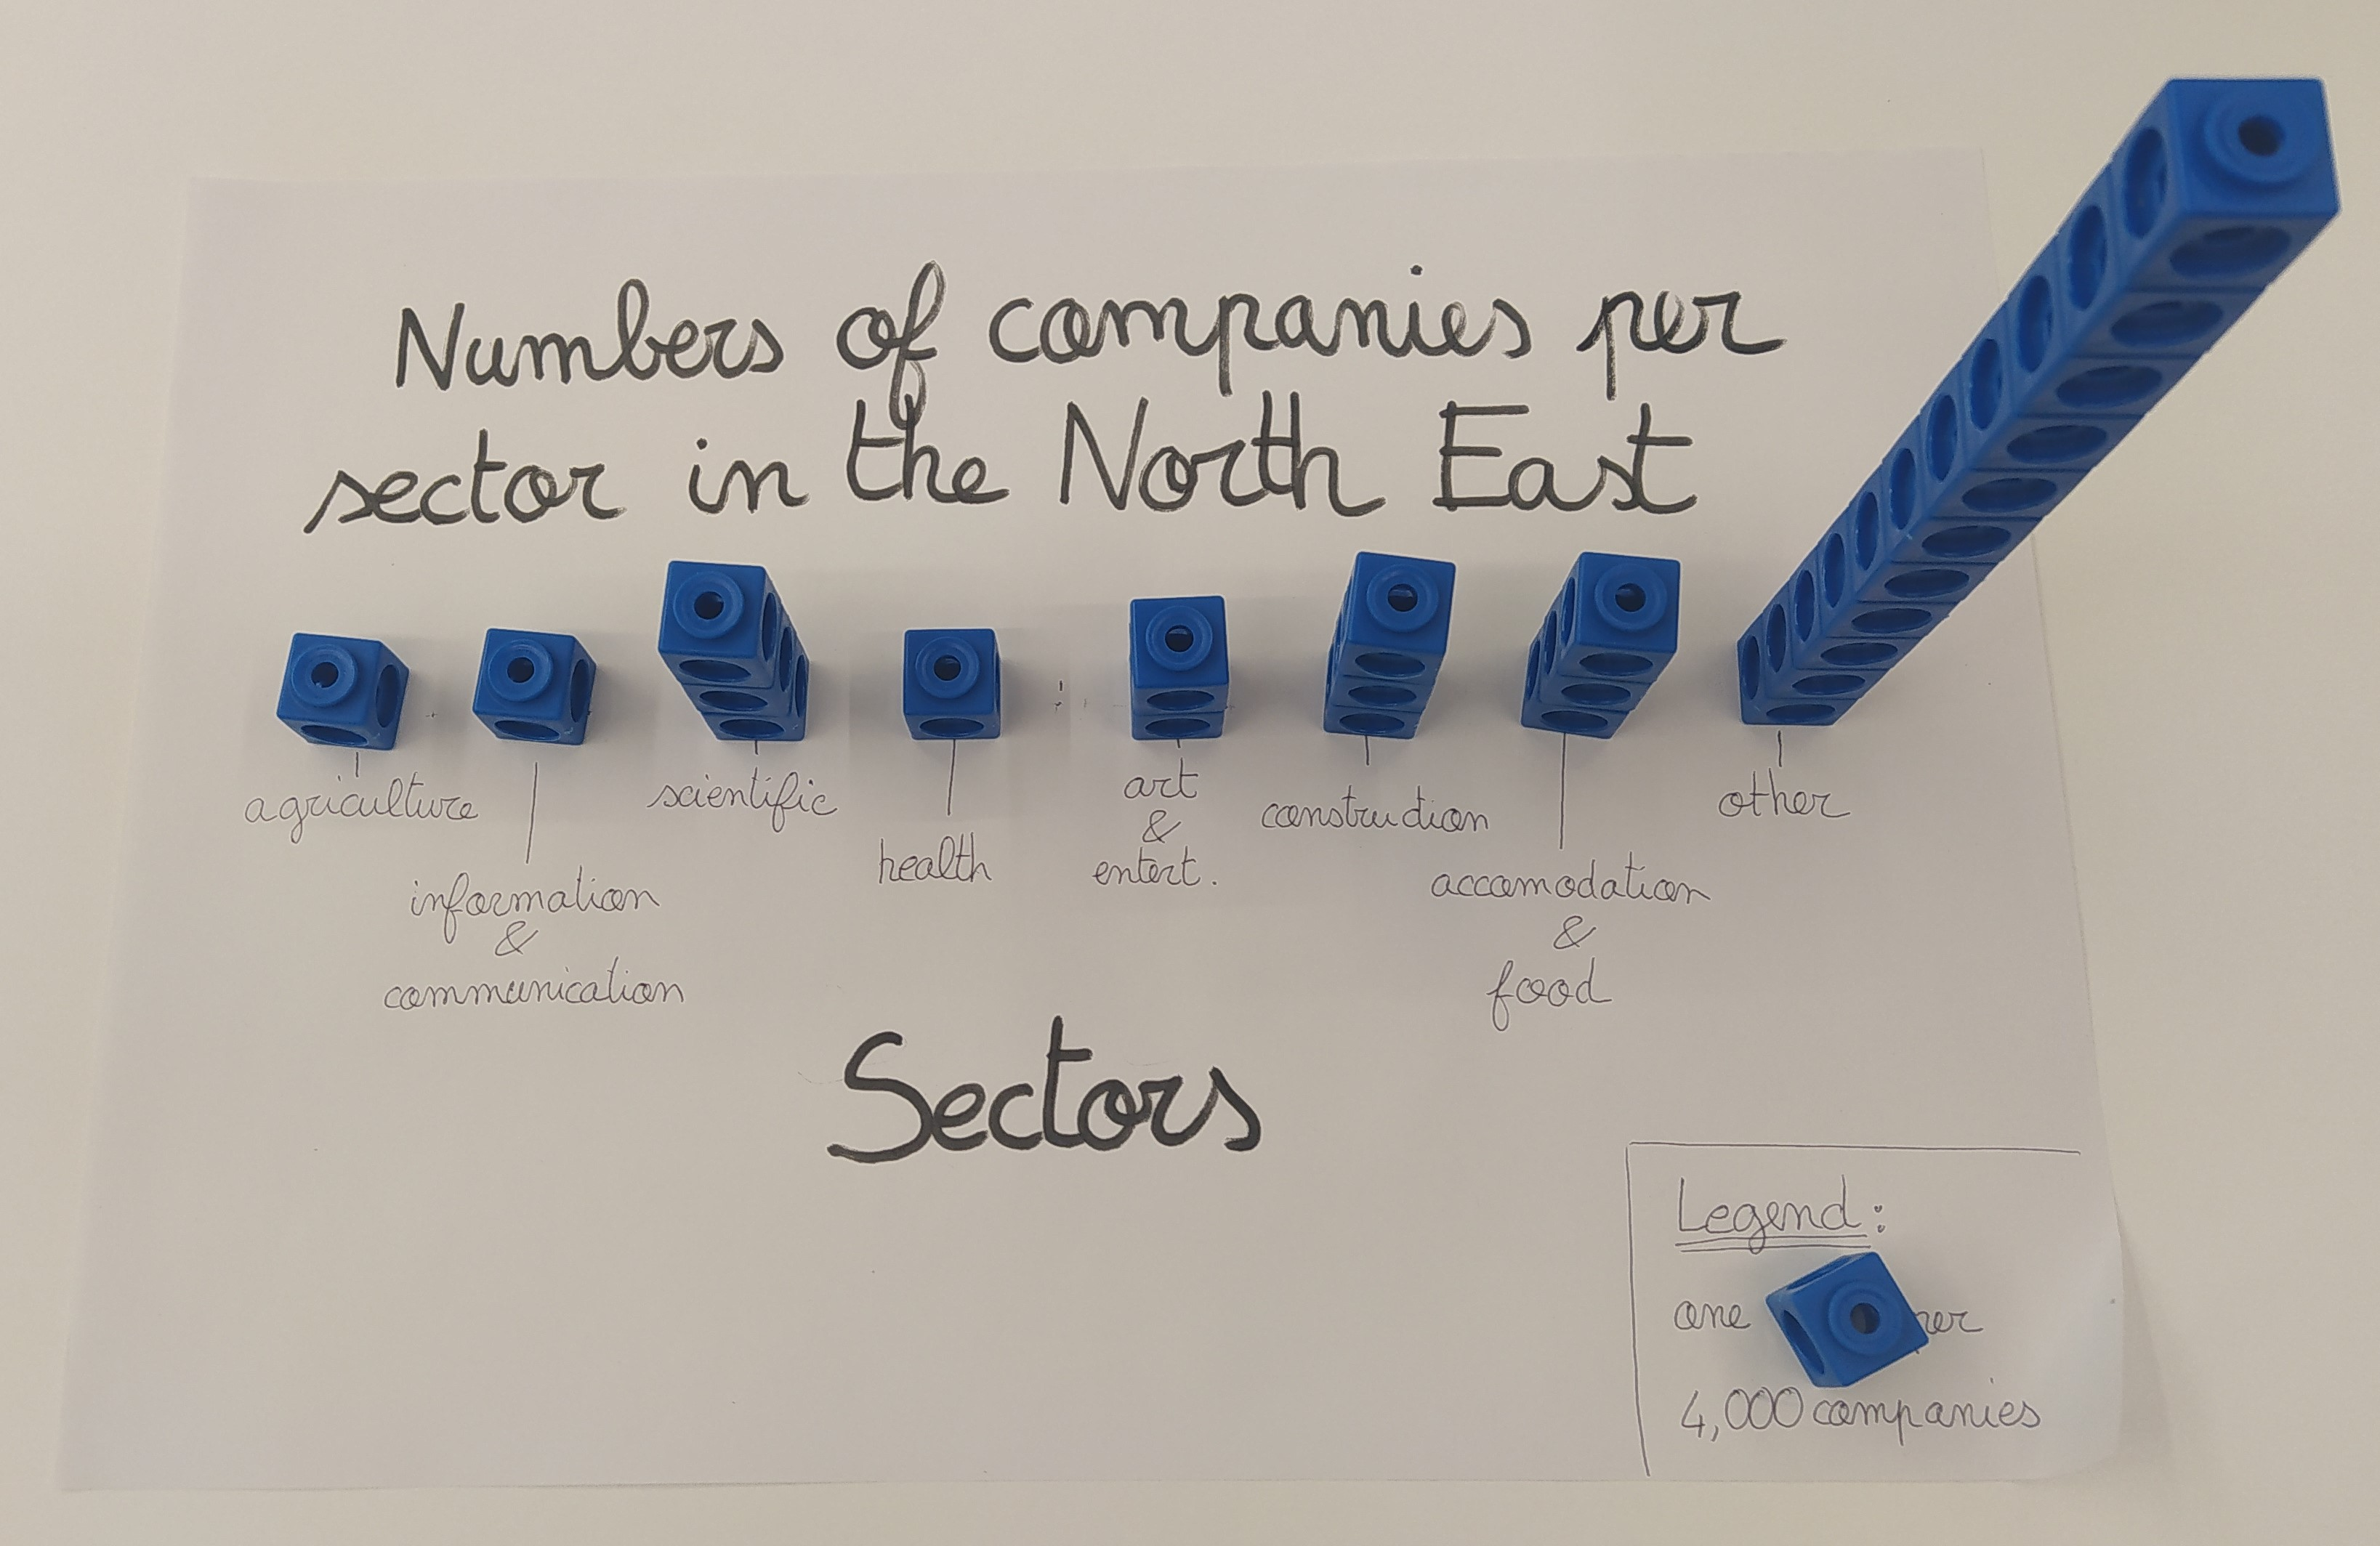
\includegraphics[width=.5\linewidth]{img/exe1-1.jpg}
    % \caption{Expected result for the exercise 1.1}
    % \label{fig:exe1-1}
\end{figure}

\subsection{Nothumberland vs Newcastle}

Create a representation comparing the number of companies per sector between Newcastle and Nothumberland.\\

Before proceeding to the next exercise, share your work with a demonstrator to receive feedback and guidance.\\

\underline{Expected result}
\\
\\
\\
\\
\\

\begin{figure}[h!]
    \centering
    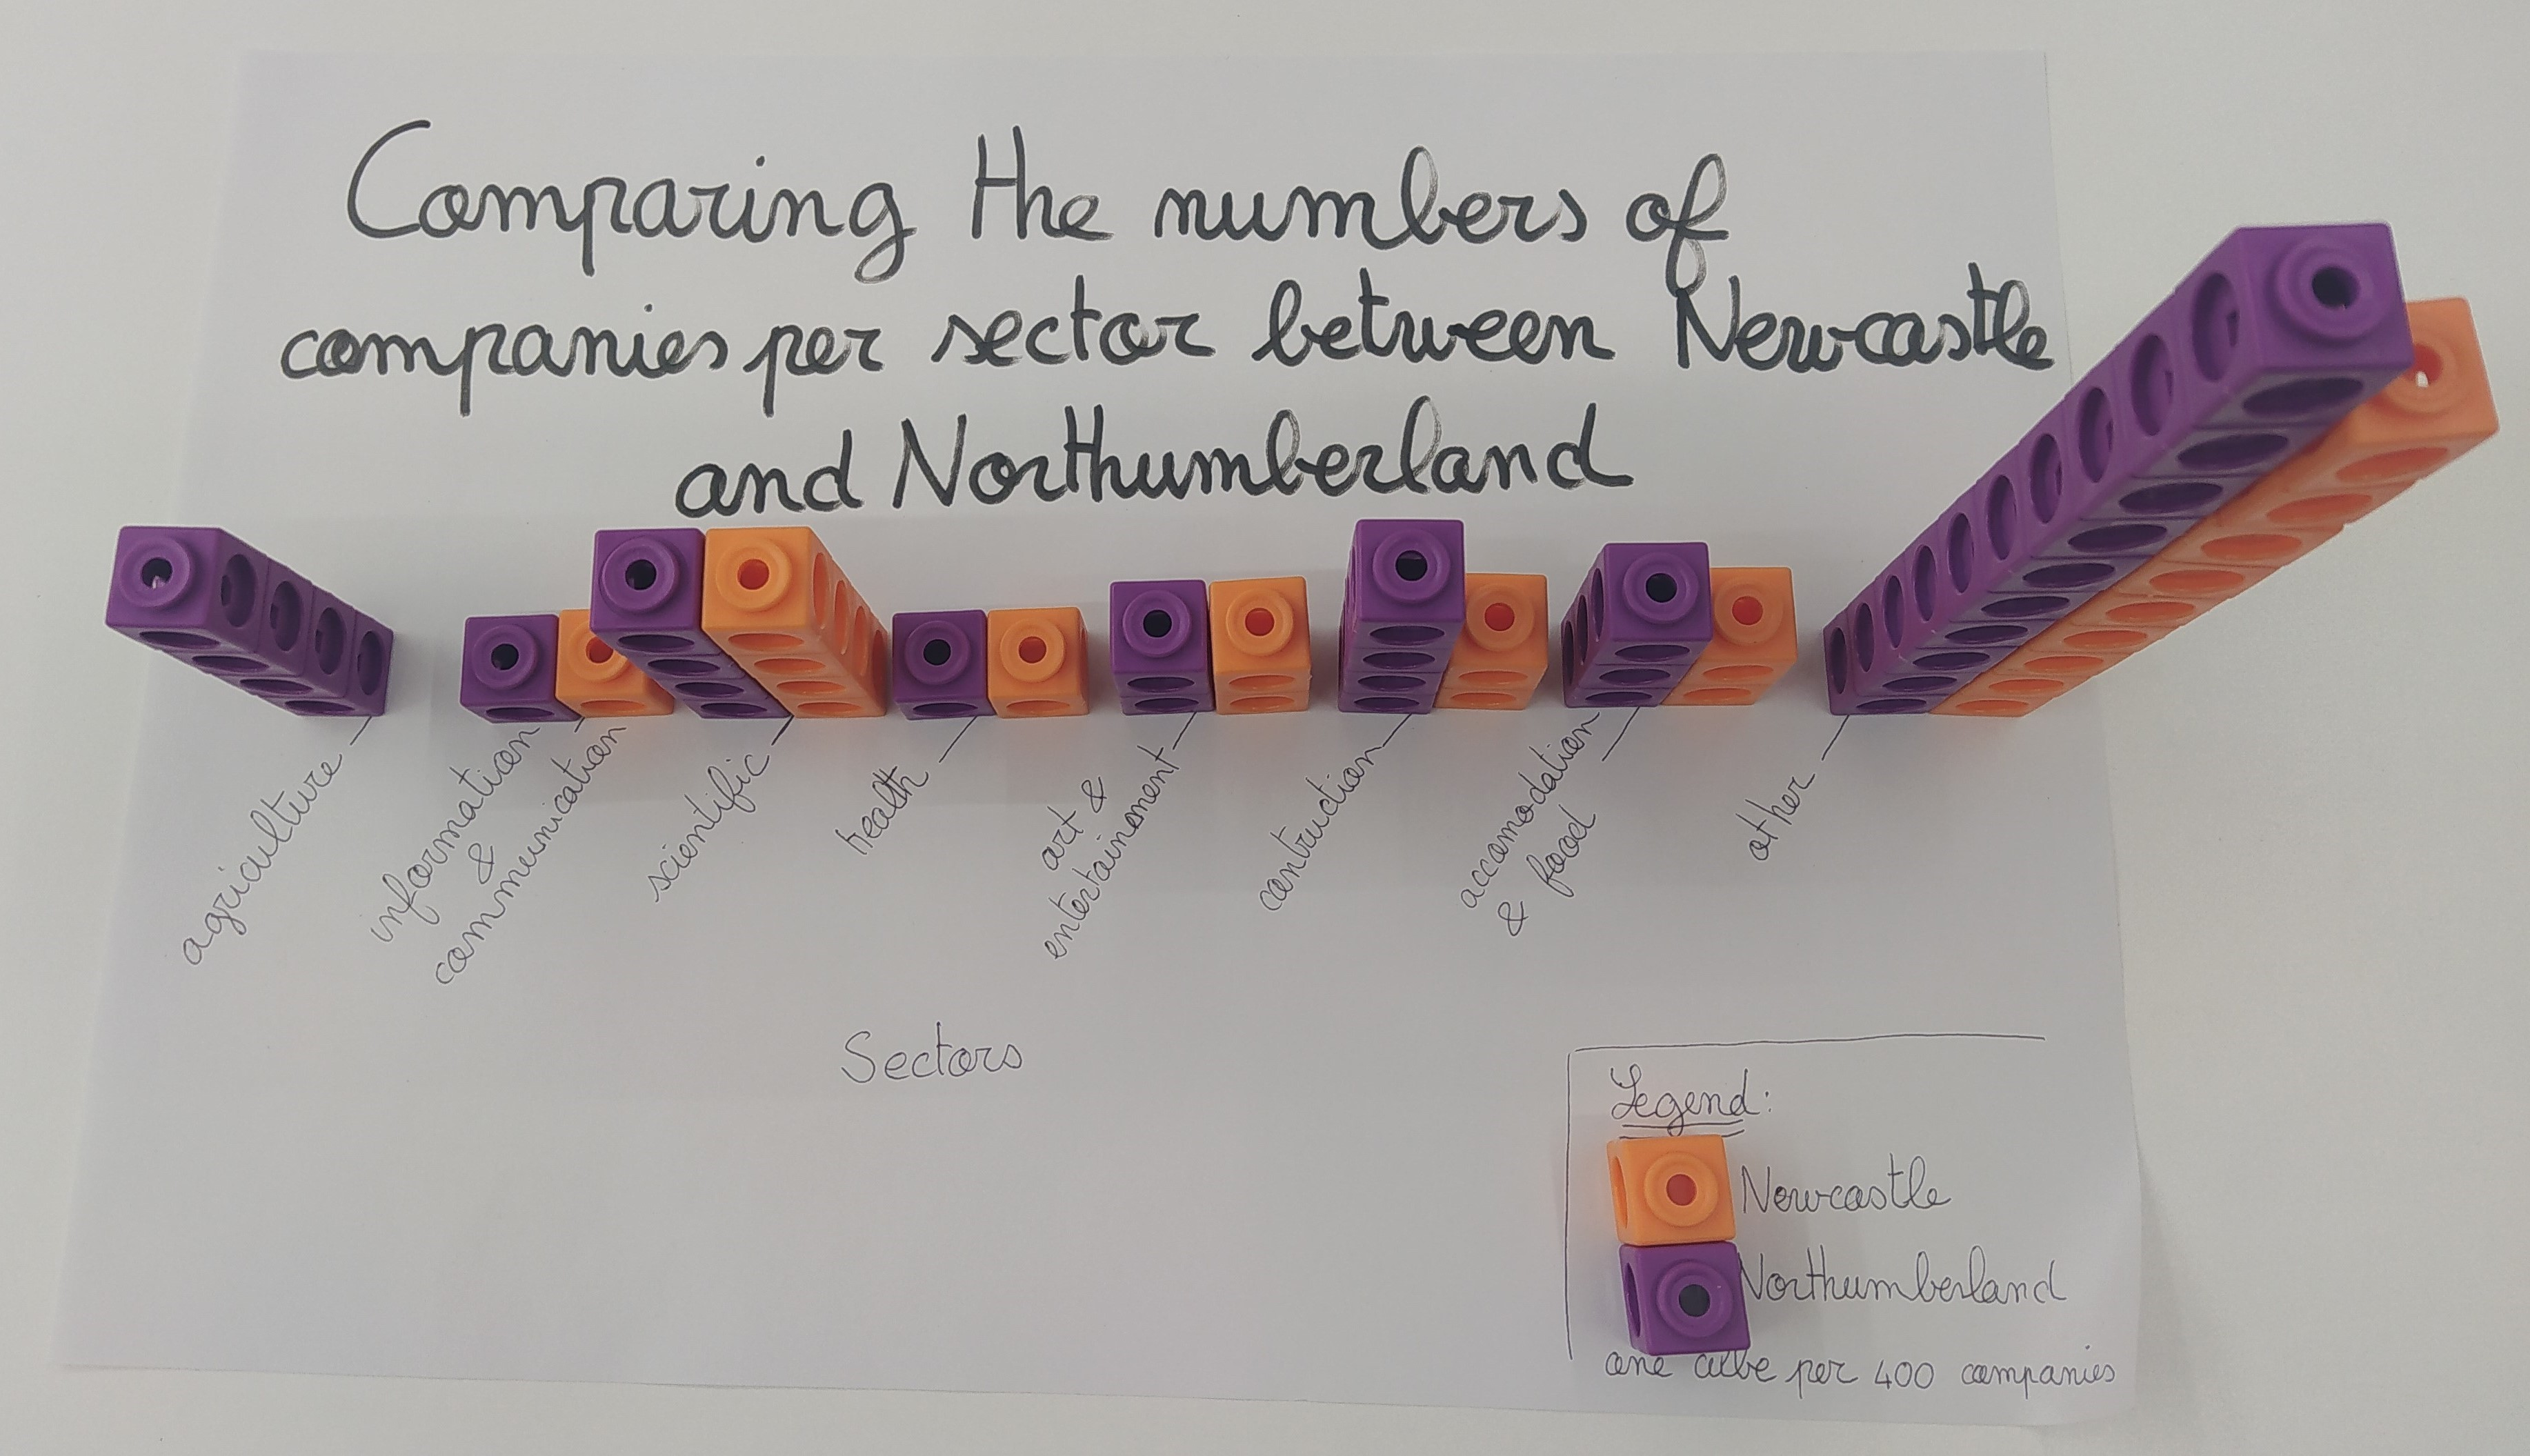
\includegraphics[width=.6\linewidth]{img/exe2-1.jpg}
    % \caption{Expected result for the exercise 1.2}
    % \label{fig:exe2-1}
\end{figure}

\subsection{Picture of the North East industrial landscape}

Represent the information of your choice based on the North East companies data.\\

Submit a picture of your completed visualization to \href{mailto:alma.cantu@newcaslte.ac.uk}{alma.cantu@newcastle.ac.uk}. The best visualizations will be selected for printing and exhibition on the 4\textsuperscript{th} floor of the USB.\\
\\

Lastly, make sure to erase any drawings on the transparent sheets and return all materials to their respective storage boxes.

\end{document}